\documentclass[problem]{mcs}

\begin{pcomments}
  \pcomment{CP_coloring}
  \pcomment{first part appears as MQ_coloring_short}
  \pcomment{soln edited ARM 3/27/14}  
\end{pcomments}

\pkeywords{
  coloring
  cycle
  chromatic_number
  subgraph
  K_4
  complete_graph
}

%%%%%%%%%%%%%%%%%%%%%%%%%%%%%%%%%%%%%%%%%%%%%%%%%%%%%%%%%%%%%%%%%%%%%
% Problem starts here
%%%%%%%%%%%%%%%%%%%%%%%%%%%%%%%%%%%%%%%%%%%%%%%%%%%%%%%%%%%%%%%%%%%%%

\begin{problem}

\begin{problemparts}

\problempart

Determine a valid coloring of the graph shown in
Figure~\ref{fig:to_color} using as few colors as possible.  (Simply
write your proposed color for each vertex next to that vertex.  You
may use $R$ for red, $G$ for green, etc.)

\begin{figure}[h]
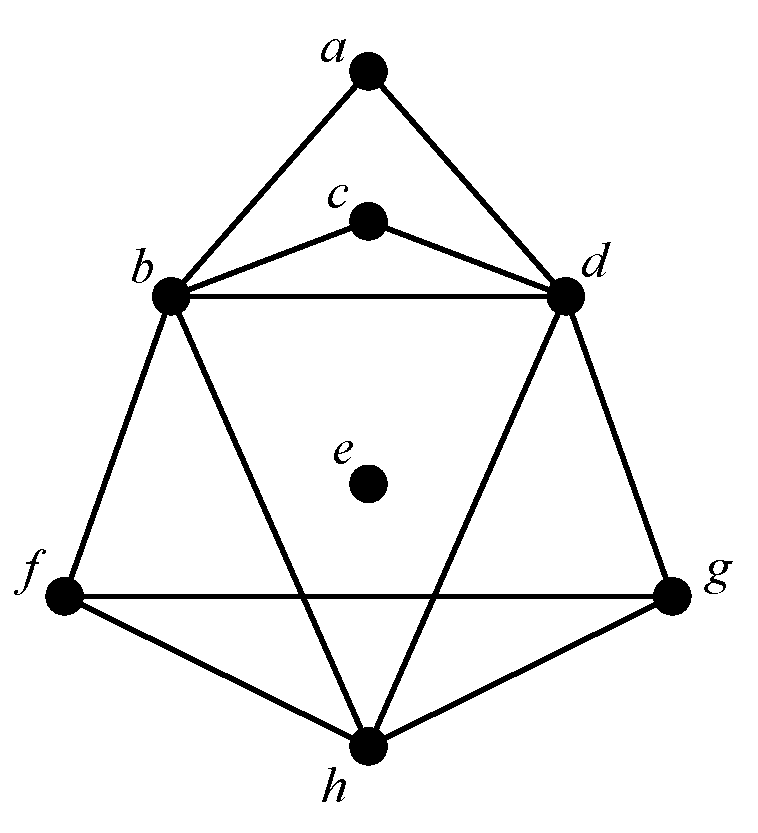
\includegraphics[width = 2in]{MQ_coloring}
\caption{\label{fig:to_color}}
\end{figure}

%\examspace[1in]

\begin{solution}
There are $K_3$'s---triangles---in the graph, so at least three colors
will be needed.  Three colors are all that's needed, as illustrated in
Figure~\ref{fig:colored}.

This 3-coloring was derived by starting with the triangle $abda$.  All
of its vertices must be colored differently, so assign red to $a$,
blue to $b$, and green to $d$.  The length three cycle $bdhb$ now
forces $h$ to be colored red.  $f$ must now be colored green and $g$
must be colored blue.  The coloring is valid so far.  $c$ is adjacent
to a blue vertex and a green vertex, and no others, it must be colored
red.  Finally, $e$ is not adjacent to any other vertices, so it can be
assigned any of the three colors.  There is no pair of like-colored
adjacent vertices, so this coloring is valid.

\begin{figure}[h]
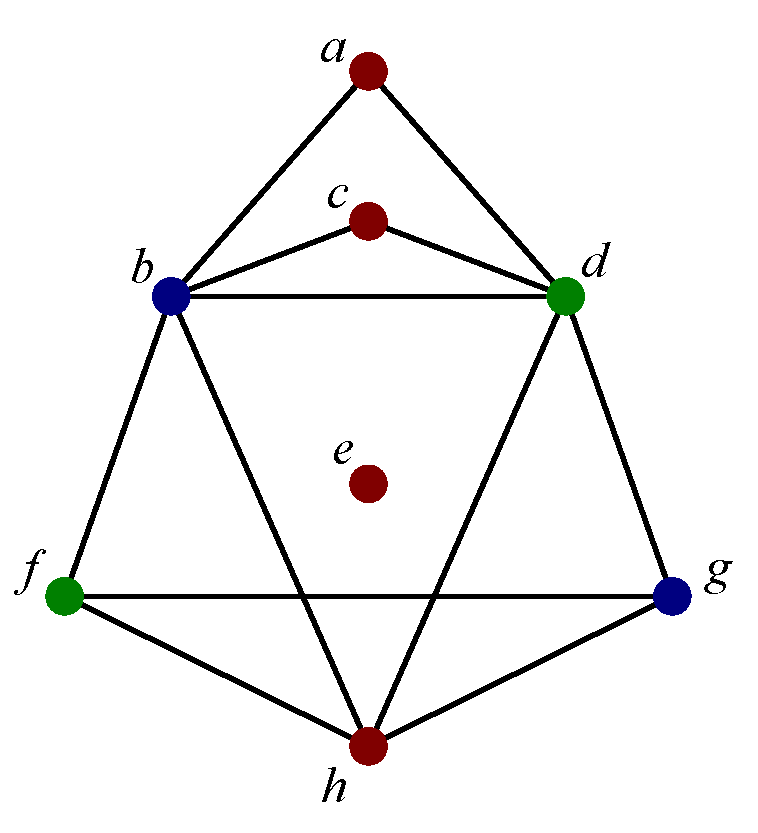
\includegraphics[width = 2in]{MQ_coloring_sol}
%\graphic{MQ_coloring_sol}
\caption{A valid coloring.}
\label{fig:colored}
\end{figure}
\end{solution}

\problempart
What is the chromatic number of the graph?

\begin{center}
\exambox{0.5in}{0.5in}{-0.5in}
\end{center}

\begin{solution}
Three.  As shown above, three colors are necessary and sufficient.
\end{solution}

\problempart Is it possible to increase the chromatic number of the
graph by adding just one edge?  If yes, state which new edge would do
the trick.  If no, explain why.

\examspace[1in]

\begin{solution}
Certainly.  There are a few possibilies.  For instance, adding
$\edge{a}{c}$ creates a subgraph isomorphic to $K_4$.  Since
$\chi(K_4)=4$, the resulting graph would have a chromatic number of at
least four---exactly four, in fact.
\end{solution}

\problempart Is it possible to decrease the chromatic number of the
graph by removing just one edge?  If yes, state which edge could be
removed to do the trick.  If no, explain why.

\examspace[1in]

\begin{solution}
No.  No matter which edge is removed, the graph will still contain a
triangle.  The chromatic number of the graph would thus still be at
least three, and hence exactly three since the 3-coloring above would
still be valid.
\end{solution}

\end{problemparts}
\end{problem}

\endinput
